\clearpage

\titlegame{Pacman}
\begin{figure}[h]
 \centering
 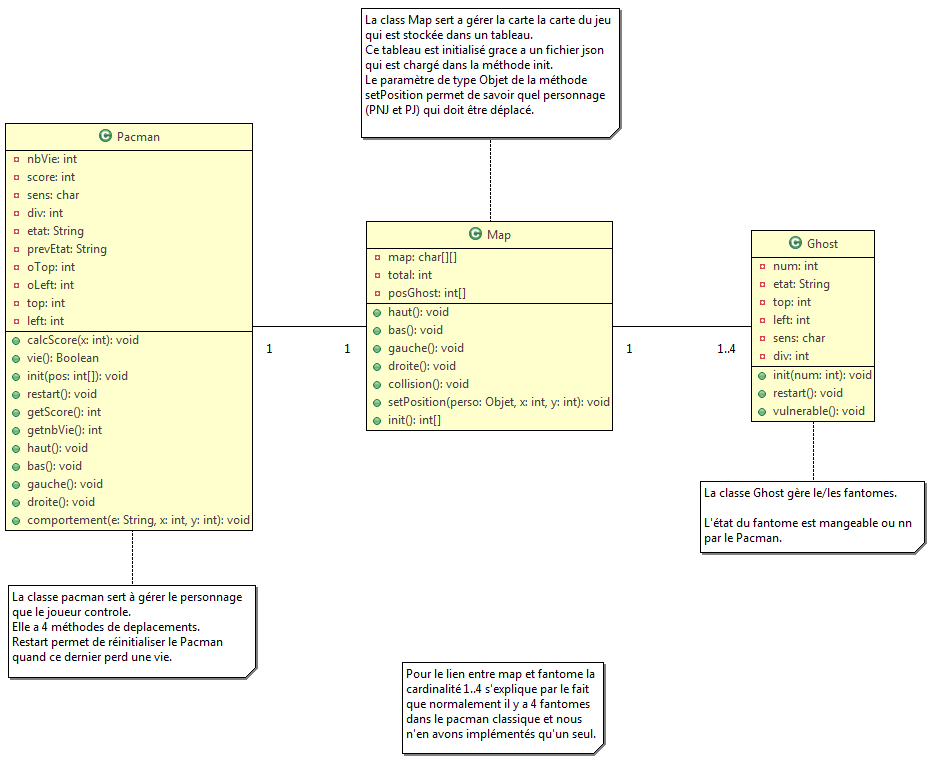
\includegraphics[width=\textwidth]{../umls/UML_images/Pacman/class} \hfill
 \caption{Diagramme de classe de Pacman}
\end{figure}

\begin{figure}[h]
 \centering
 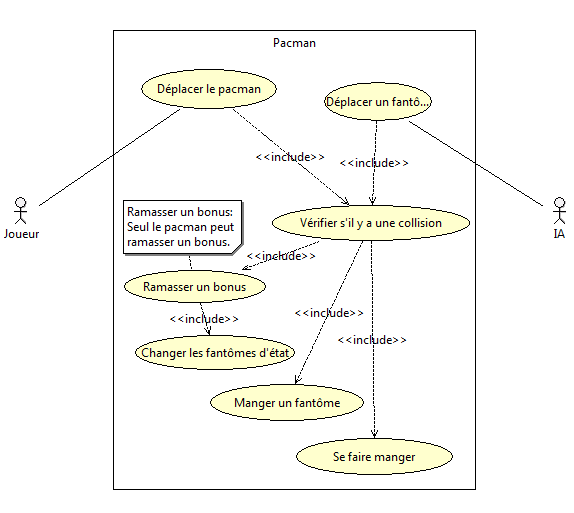
\includegraphics[width=10cm]{../umls/UML_images/Pacman/utilisation}
 \caption{Diagramme d'utilisation de Pacman}
\end{figure}

\begin{figure}[h]
 \centering
 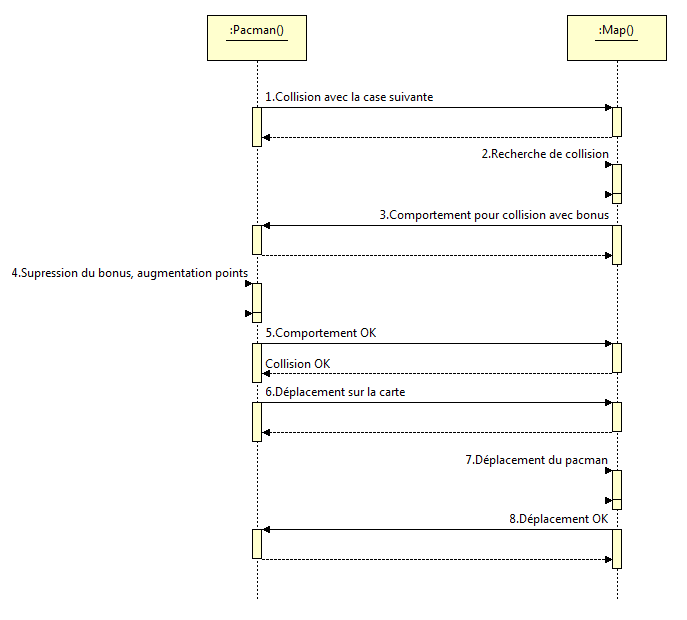
\includegraphics[width=9cm]{../umls/UML_images/Pacman/sequence} \hfill
 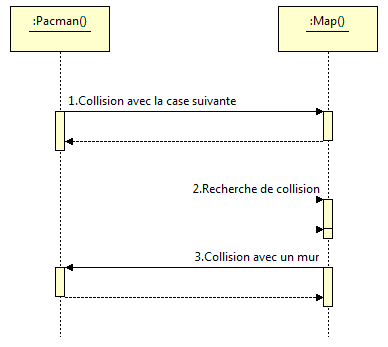
\includegraphics[width=6cm]{../umls/UML_images/Pacman/sequence2} \hfill
 \caption{Diagrammes de séquence de Pacman}
\end{figure}



% \clearpage
% 
% \begin{figure}[h]
%  \centering
%  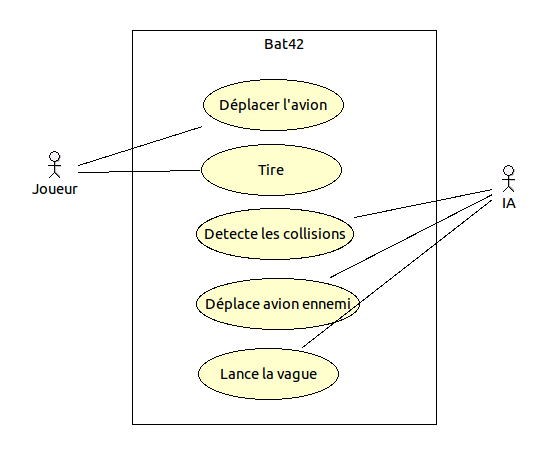
\includegraphics[width=7cm,height=7cm]{../umls/UML_images/Bat42/utilisation} \hfill
%  \includegraphics[width=8cm]{../umls/UML_images/Bat42/sequence} \hfill
%  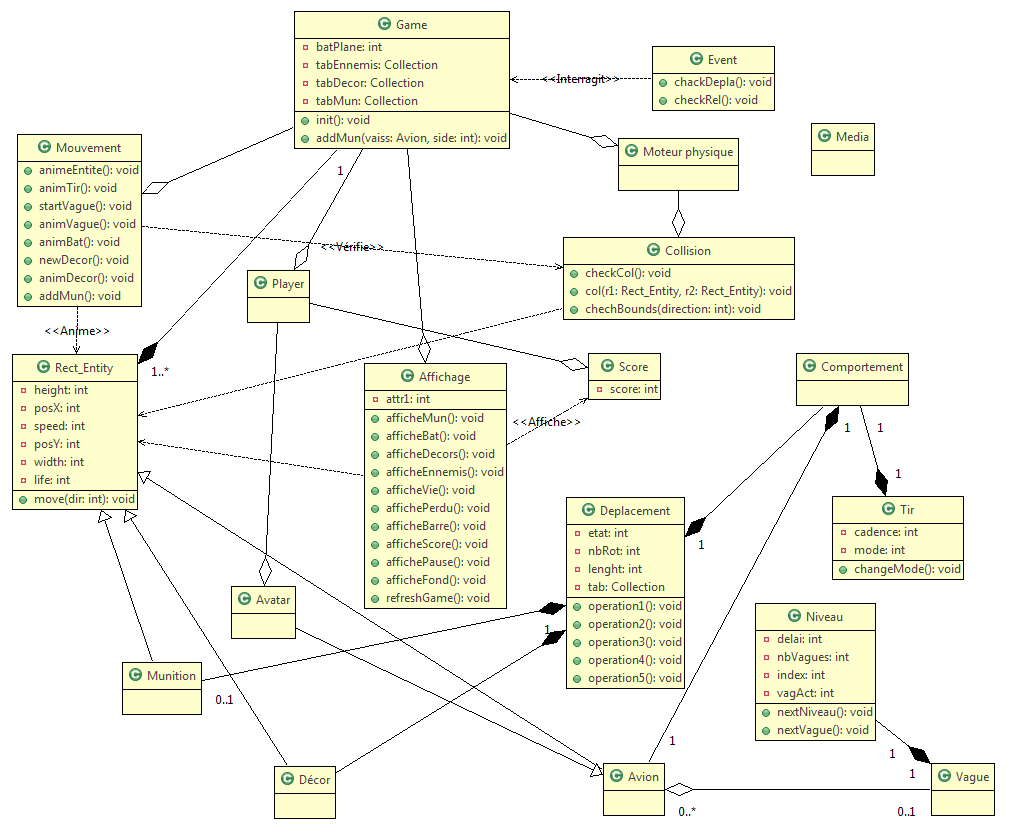
\includegraphics[height=8cm]{../umls/UML_images/Bat42/class} \hfill
%  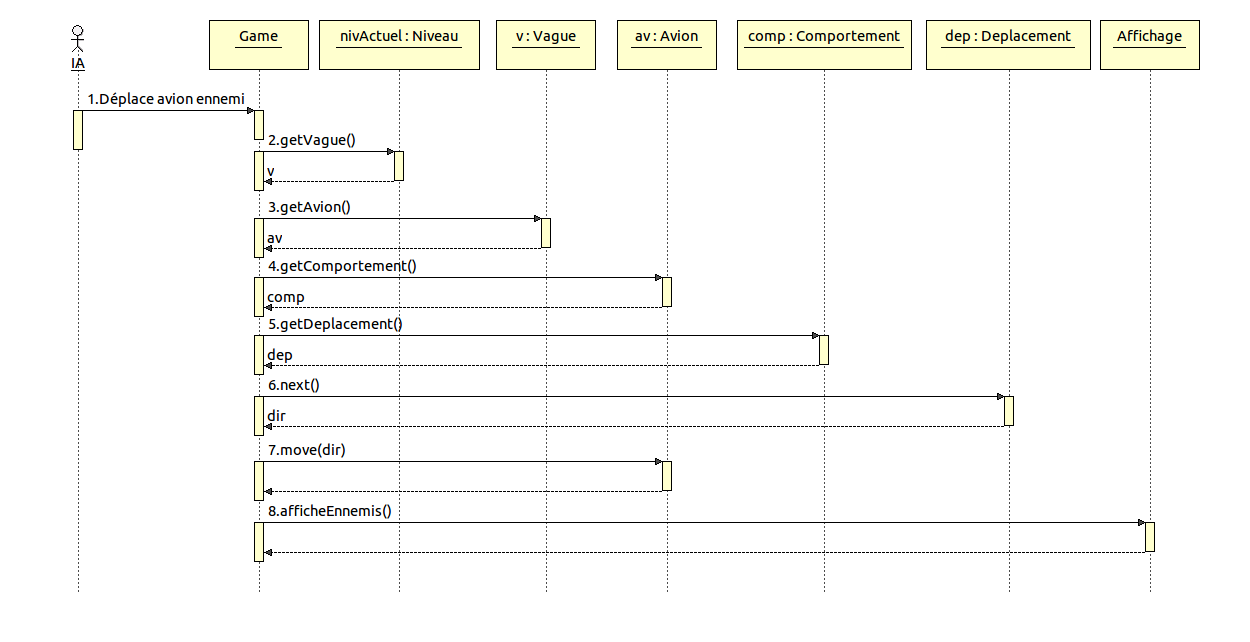
\includegraphics[height=7cm]{../umls/UML_images/Bat42/sequenceIA} \hfill
%  \caption{En haut à droite, le diagramme d'utilisation de 1942; en bas à droite, son diagramme de classe ; sur la droite, 2 diagrammes de séquence}
% \end{figure}


% \titlegame{Volley}
%  \uml{Volley/utilisation}{Diagramme de cas d'utilisation du jeu de volley}
%  \uml{Volley/class}{Diagramme de classe du jeu de volley}
%  \uml{Volley/sequence}{Diagramme de séquence du jeu de volley}
%  \uml{Volley/sequence2}{Diagramme de séquence du jeu de volley}
%  \uml{Volley/sequence3}{Diagramme de séquence du jeu de volley}
%  \uml{Volley/sequence4}{Diagramme de séquence du jeu de volley}
% 

\clearpage
\titlegame{Course}

\begin{figure}[h]
 \centering
 \includegraphics[width=\textwidth]{../umls/UML_images/course/sequence} \hfill
 \caption{Diagramme de séquence du jeu de course}
\end{figure}

\begin{figure}[h]
 \centering
 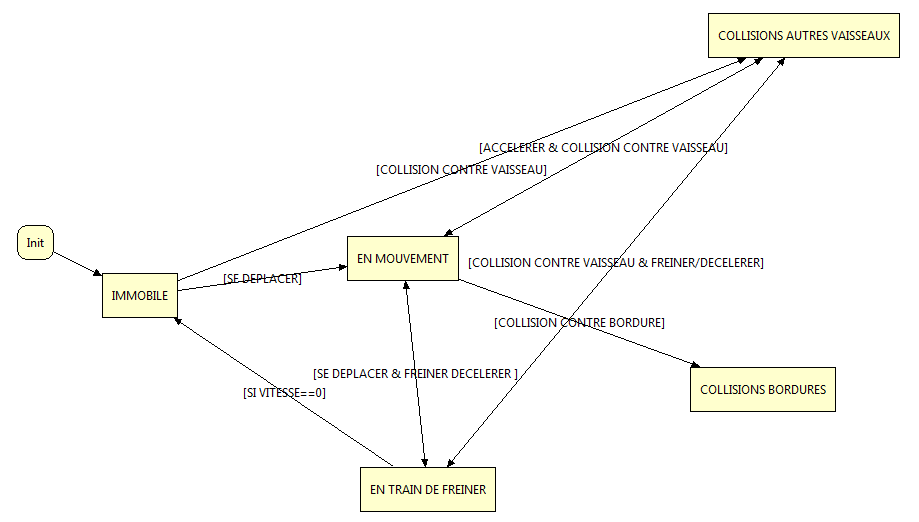
\includegraphics[width=\textwidth,height=8cm]{../umls/UML_images/course/activity} \hfill
 \caption{Diagramme d'activité du jeu de course}
\end{figure}

\begin{figure}[h]
 \centering
 \includegraphics[width=\textwidth]{../umls/UML_images/course/class} \hfill
 \caption{Diagramme de classe du jeu de course}
\end{figure}


\clearpage
\titlegame{Mario}

\begin{figure}[h]
 \centering
 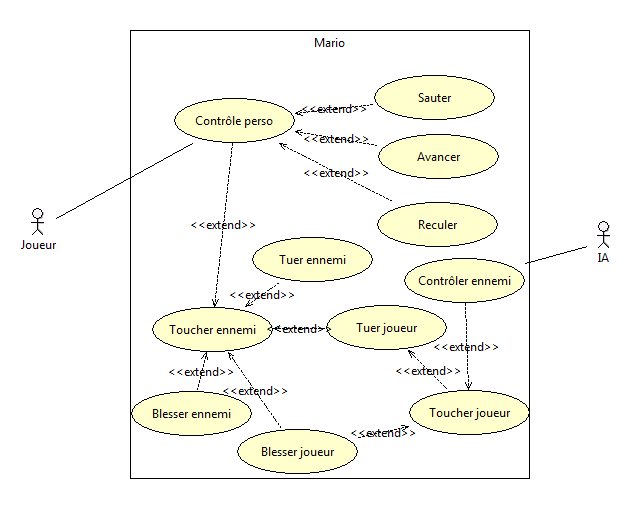
\includegraphics[width=\textwidth]{../umls/UML_images/Mario/Utilisation} \hfill
 \caption{Cas d'utilisation de Mario}
\end{figure}

\begin{figure}[h]
 \centering
 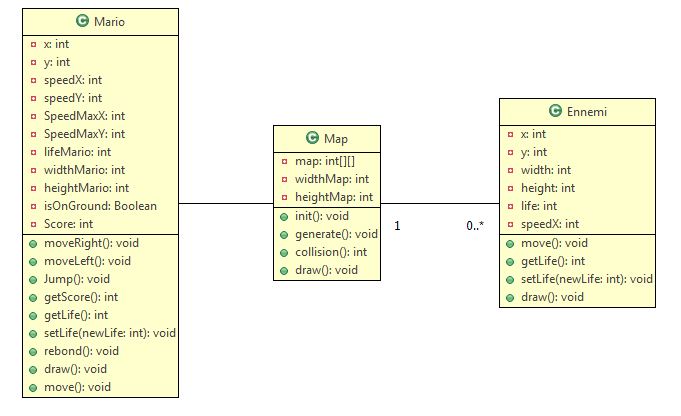
\includegraphics[height=9cm]{../umls/UML_images/Mario/Class} \hfill
 \caption{Diagramme de classes de Mario}
\end{figure}

\begin{figure}[h]
 \centering
 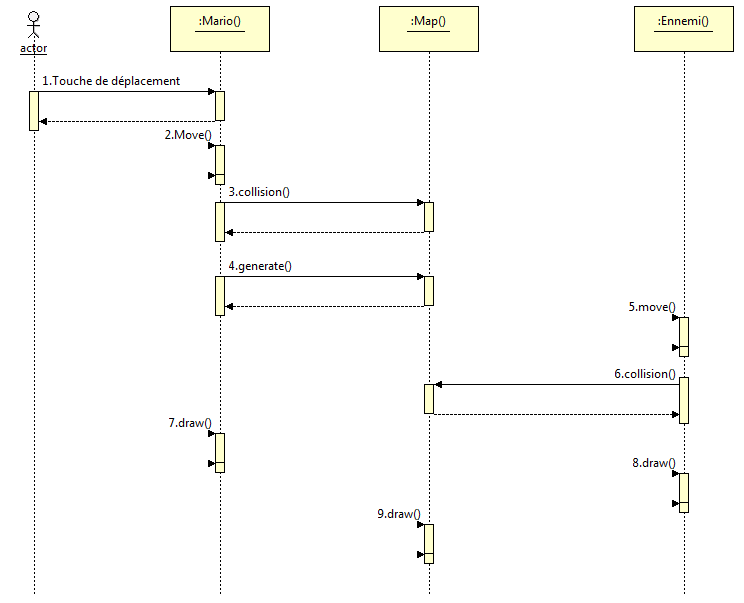
\includegraphics[height=11.5cm]{../umls/UML_images/Mario/Sequence} \hfill
 \caption{Diagramme de séquence de Mario}
\end{figure}


% 
% \titlegame{Watch'N'Droid}
%  \uml{WatchNDroid/class}{Diagramme de classe du jeu Watch'N'Droid}
%  \uml{WatchNDroid/sequence}{Diagramme de séquence du jeu Watch'N'Droid}
% 
\clearpage
\titlegame{Billard}

\begin{figure}[h]
 \centering
 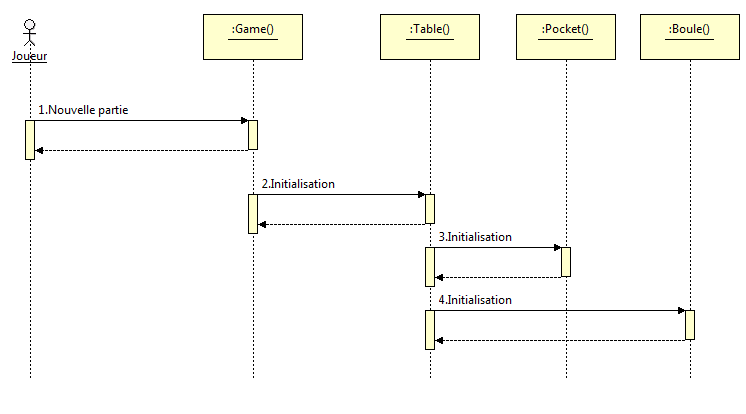
\includegraphics[height=6.5cm]{../umls/UML_images/Billard/sequence1} \hfill
 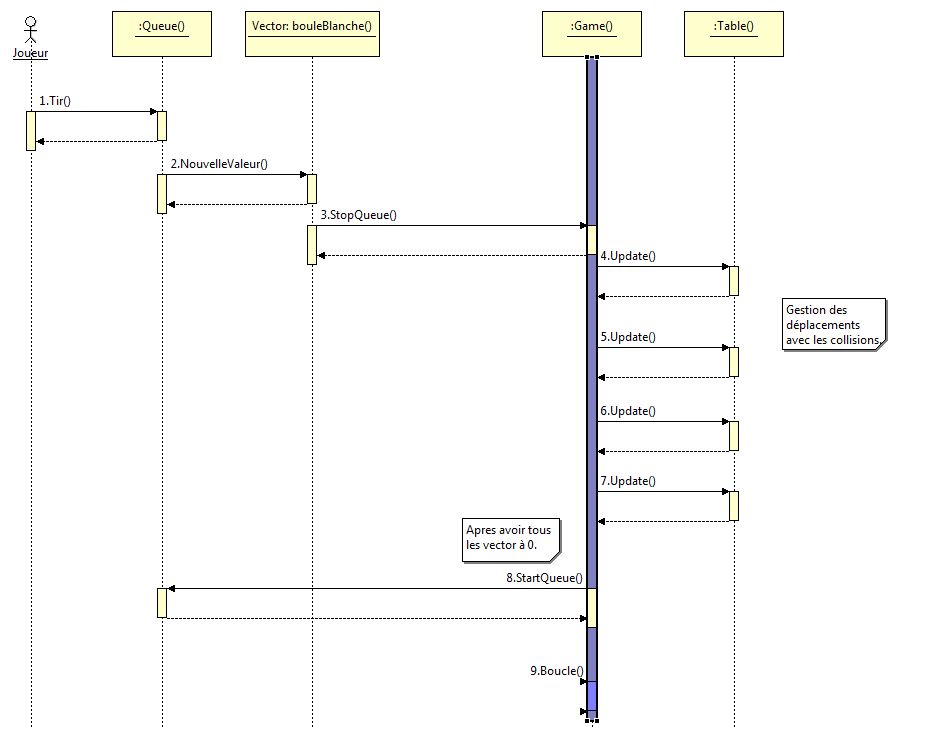
\includegraphics[height=11cm]{../umls/UML_images/Billard/sequence2} \hfill
 \caption{Diagrammes de séquence du billard}
\end{figure}

\begin{figure}[h]
 \centering
 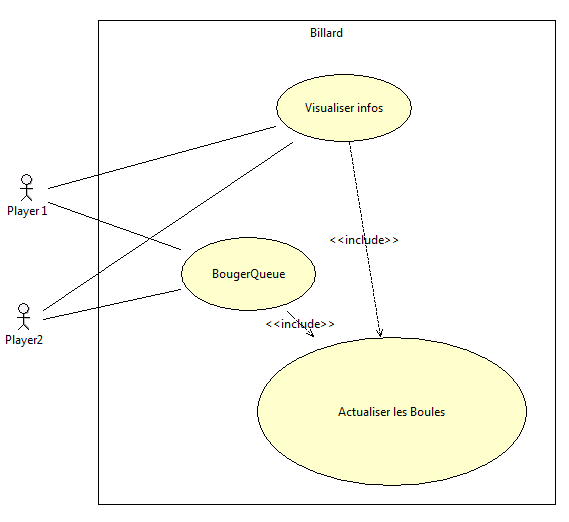
\includegraphics[height=7cm]{../umls/UML_images/Billard/utilisation} \hfill
 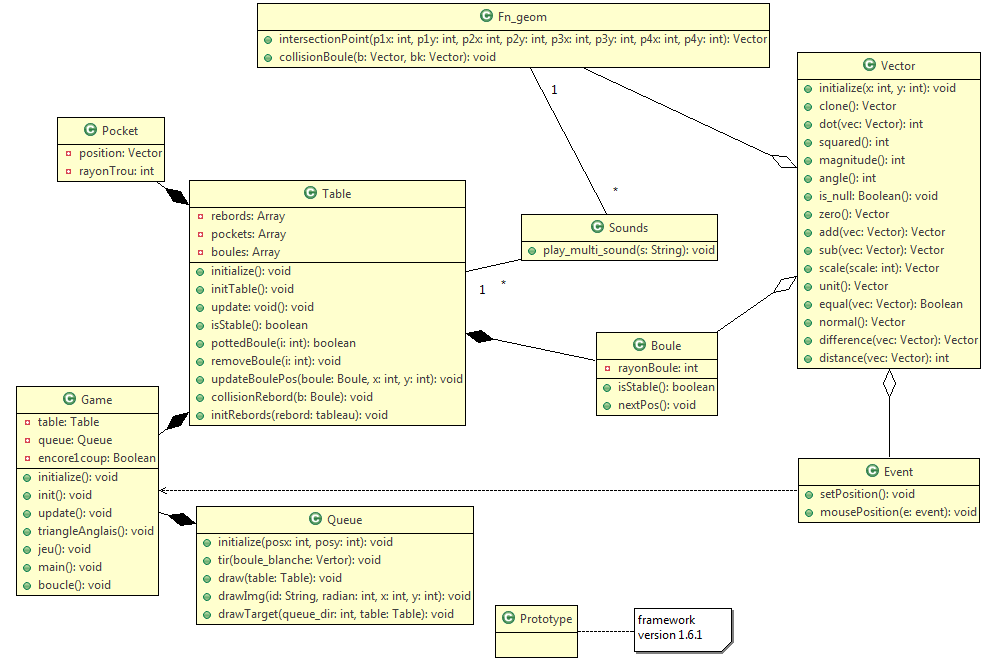
\includegraphics[width=\textwidth,height=12cm]{../umls/UML_images/Billard/class} \hfill
 \caption{En haut, les cas d'utilisation du billard ; en bas, son diagramme de classes}
\end{figure}


%  \uml{Billard/utilisation}{Diagramme de cas d'utilisation du jeu de billard}
%  \uml{Billard/class}{Diagramme de classe du jeu de billard}
%  \uml{Billard/sequence1}{Diagramme de séquence du jeu de billard}
%  \uml{Billard/sequence2}{Diagramme de séquence du jeu de billard}
% 
% 

\clearpage
\titlegame{Gestion}

\begin{figure}[h]
 \centering
 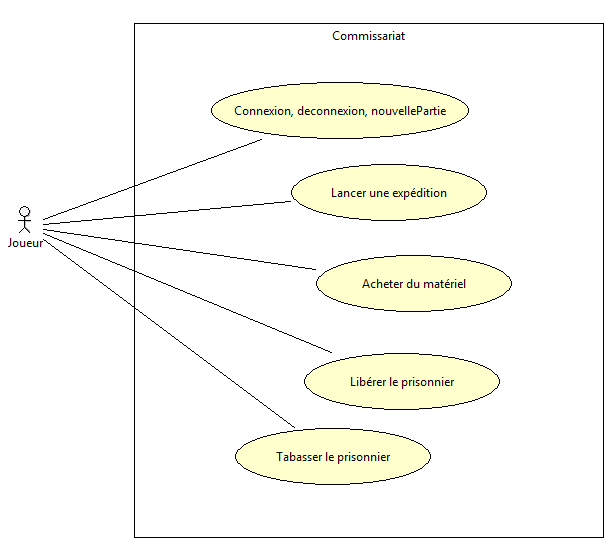
\includegraphics[width=\textwidth]{../umls/UML_images/Commissariat/utilisation} \hfill
 \caption{Cas d'utilisation du jeu de gestion}
\end{figure}

\begin{figure}[h]
 \centering
 \includegraphics[width=\textwidth]{../umls/UML_images/Commissariat/class} \hfill
 \caption{Diagramme de classes du jeu de gestion}
\end{figure}